\subsection{Overview of the architecture}
Tinker system has to deal with challenges at different levels from hardware interface to artificial intelligence. Thus, a multi-level, distributed architecture based on ROS is employed to meet such requirement. The hardware layer contains a embedded board driving motors and preprocessing odometry data. The hardware-communication layer is responsible for controlling the motors and acquiring information from the sensors. The output of the hardware layer is ROS-compatible sensor images including camera image, point cloud and multiple other topics. The logic layer is responsible for providing basic functions of a robot such as manipulation, navigation, human tracking, object recognition, speech recognition and synthesis etc. The decision layer listens to topics published by the logic layer and makes decision for the next high-level action to accomplish the task.

\subsubsection{The hardware layer}
\ 

The power management we use are:
\begin{enumerate}
	\item Calf electric vehicle battery for center processor and chassis.
	\item Dji battery with step-down or up transformer for the other equipments.
\end{enumerate}

The mechanism we use are:
\begin{enumerate}
    \item DJI M3058P19 motors for driving the chassis and the platform.
    \item Universal-Robots UR5 robot arm for accessing objects.
    \item Robotiq-G85 mechanical claw.
\end{enumerate}

Sensors we use are:
\begin{enumerate}
    \item Hokuyo URG04LX laser scanner for navigation
    \item Hokuyo UTM30 laser scanner for navigation
    \item VEILODYNE VLP16 multi-laser scanner for navigation and hunamn tracking
    \item Kinect v2 depth camera for navigation and object detection
    \item Realsense D435I camera for object recognition and detection
    \item Xsense MTi-10 nine-axis IMU
    \item Encoder on motors for motor controlling
    \item Laser transmitter and receiver sensor for confirming the grasping
\end{enumerate}

\subsubsection{The hardware-communication layer}
\ 

The hardware communication layer must be highly scalable to quickly install and remove different sensors and executors. All control commands of the robot are sent to the ROS nodes running on the laptop. Laptop also collect the information collected by the various sensors and control mechanical operations.
\begin{figure}[!t]
	\centering
    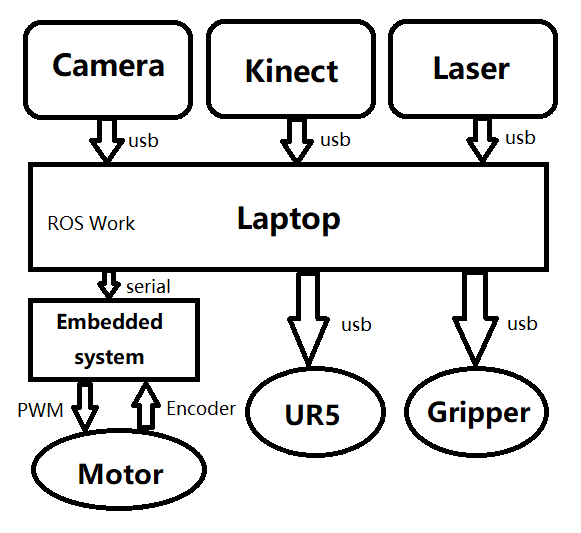
\includegraphics[scale=0.5]{commuication_arch.png}
    \caption{The architecture of the hardware-communication layer}
    \label{arch_comm}
\end{figure}

\subsubsection{The logic layer}
\ 

Most important robot functions are implemented in this layer. The main components in this layer include:
\begin{enumerate}
    \item Navigation: Mapping, localization, route-planning and collision avoidance
    \item Vision: Human recognition, object recognition and their tracking.
    \item Speech: Speech recognition and synthesis
    \item Manipulation: Robot arm planing with feedback from vision and laser
\end{enumerate}

\subsubsection{The decision layer}
\ 

Task planning is done in decision layer. For different tasks, modules in decision layer run as state machine. They integrate different information from the low layer to judge the state they are in and then give different orders or make different responses. Each module deal with a single task, sharing the common information from the lower layers.

